\chapter{Résumé détaillé}

\selectlanguage{french}

\section{Introduction : robots, interaction et connaissances}
\label{chapt|introduction}

Nao a été aperçu jouant avec des enfants autistes, Justin tapote sur la boite
de chocolat en poudre pour préparer le petit-déjeuner, des robots PR2 nous
amènent des bières et distribuent du popcorn dans les laboratoires, tandis que
Rosie s'occupe des crêpes pour le goûter : si ces expériences récentes, mises
en place un peu partout dans les laboratoires de robotique nous dise une chose,
c'est que la robotique de service est en train de quitter le domaine de la
science-fiction, des rêves, des fantasmes et s'apprête à frapper à la porte de
notre quotidien.

\begin{figure}[!h]
    \centering
    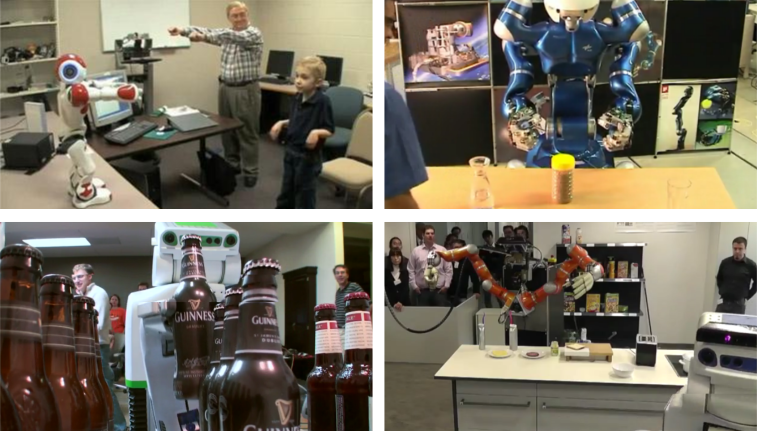
\includegraphics[width=0.8\columnwidth]{intro/everyday_robots.pdf}

    \caption*{Nao, Justin, PR2, Rosie: les robots jouent avec les enfants,
    préparent des chocolats chauds, décapsulent les bières et font sauter les
crêpes. Pour l'instant en laboratoire, sans interactions très avancées avec les
hommes. Que leur manquent-ils pour s'inviter dans nos maisons ?}

    \label{fig|everyday-robots}
\end{figure}

Des progrès considérables ont été accomplis au niveau de la perception des
robots : les caméras et les lasers sont aggrégés dans des pseudo-capteurs
renvoyant des informations de haut-niveau : reconnaissance de visages,
localisation et cartographie SLAM, posture dynamique des hommes... Permettre à
un robot de comprendre son environement est aujourd'hui un défi où deux
facettes se mèlent : reconstruire en continu un monde géométrique et dynamique
cohérent ; abstraire ce même monde en une représentation symbolique adaptée au
raisonnement logique.

La résolution de ce premier défi, auquel cette thèse tente de contribuer, n'est
cependant pas suffisante pour permettre une interaction entre hommes et robots.
Le robot auquel nous pensons vit dans le monde réel, un monde pour et avec des
humains. Notre robot doit acquérir des compétences sociales, il doit pouvoir
considérer les hommes autour de lui non seulment comme des entités physiques
(...sur lesquelles ils ne faut pas rouler par exemple), mais aussi et surtout
comme des entités intelligentes, dotées d'une individualité propre et unique.

Le robot doit pouvoir non seulement représenter son environement, représenter
son propre état mental, mais aussi tenter de deviner et de représenter l'état
mental, les connaissances des autres agents avec lesquels il interagit. Et ces
modèles, il faut ensuite savoir les mettre en \oe uvre pour donner corps  des
compétences sociales au premier rang desquelles se trouve la fonction de
communication.

\begin{figure}
    \centering
    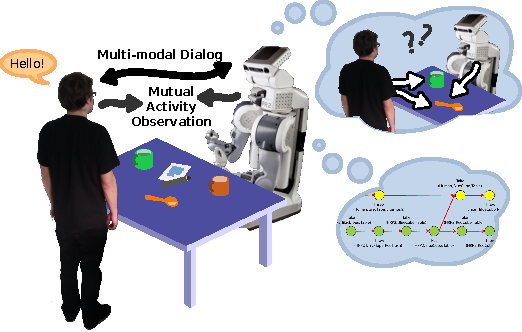
\includegraphics[width=0.9\columnwidth]{intro/grounding_robot.pdf}
    
    \caption{Le robot est plongé dans une \emph{situation}. Les source de
    connaissances sont multiples : dialogue multi-modal, observation de
    l'environement et des activités de l'homme, capacités internes de planification
    et de raisonnement symbolique. Le robot raisonne non seulement de son propre
    point de vue, mais en se projettant à la place des autres agents.}

    \label{fig|hri-dec}
\end{figure}

La figure~\ref{fig|hri-dec} résume les principaux aspects de l'interaction qui
nécessitent d'être traduit dans des modèles adaptés au robot. Du point de vue
du robot, plusieurs compétences cognitives sont impliquées : traitement du
dialogue (verbal et déictique : regard, posture, gestes...), acquisition et
maintient de un ou plusieurs modèles de l'environnement (non seulement du point
de vue du robot, mais aussi des points de vue de chacun des autres agents),
anticipation (quelles sont les intentions de l'humain ? Puis-je prédire ses
actions ?), planification et contrôle (comment puis-je progresser vers le but
?), suivi des activités des autres agents (est-ce que la coopération est
effective ?) et de l'avancement générale de la tâche.

Chacune de ces capacités cognitives se traduit en contraintes et besoins sur le
système de représentation de connaissances, comme nous allons le présenter
un peu après.



\subsection{Un programme}
\label{sect|challenges}

Cette brève introduction laisse deviner en négatif le programme de recherche que nous
défendons dans cette thèse, et que nous résumons ici. Nous pouvons essayer
d'articuler les trois défis liés au champ de la représentation des
connaissances dans la robotique de service et robotique-compagnon que nous
traitons dans ce travail de doctorat.

Notre premier objectif est en réalité de préciser cette notion de
\emph{représentation de la connaissance} qui est en réalité mal définie. Depuis
l'enfance de l'intelligence artificielle, depuis l'idée de \og  l'étage de la
connaissance \fg de Newell, il est admis que les systèmes intelligents ont
besoin de représenter et de manipuler de la connaissance. Mais quoi au juste ?
Il semble nécessaire de poser des fondations théoriques et pratiques solides à
cette question sur lesquelles le champ de la robotique cognitive pourrait
s'appuyer. C'est notre premier défi.

Le deuxième défi est plus technique : comment effectivement réaliser un tel
robot cognitif ? quelles sont les spécificités de la robotique (notament du
fait de l'incarnation physique du robot) ? pouvons nous aujourd'hui construire
au moins une instance d'un système cognitif adapté à l'interaction dans le
monde physique ?

Notre troisième défi se concentre sur les aspects liés à l'interaction
homme-robot. Nous affirmons que les robots appartiennent désormais à l'ensemble
des individus sociaux. Qu'est-ce que cela signifie ? quelles conséquences cela
a-t'il sur notre modèle de connaissances ? comment cela se traduit-il en
problèmatique concrète comme la compréhension du language naturel ?

Chacunes des contributions de cette thèse, résumées ci-dessous, peuvent être
rapportées à l'un de ces défis, et nous espérons qu'elles contribuent à une
meilleure compréhension de ces problématiques.

%%%%%%%%%%%%%%%%%%%%%%%%%%%%%%%%%%%%%%%%%%%%%%%%%%%%%%%%%%%%%%%%%%%%%%%%%%%%%%%

\subsection{Contributions de cette thèse}
\label{sect|contributions}

Le point de départ de cette thèse est le sentiment qu'une meilleure
compréhension des besoins en terme de connaissance des applications robotiques
en environement humain (c'est à dire, complexe, dynamiques et sémantiquement
riche) serait bénéfique à la recherche en robotique cognitive.

Se basant sur une large revue de la littérature et la formulation de plusieurs
scénarios d'interaction (dont certains ont conduit a des expériences sur les
robots), nous avons itérativement affiné la problématique de la
\emph{connaissance pour l'interaction}. La formalisation de cette problématique
est l'un des principaux résultats de ce travail : nous avons listé et organisé
en une typologie un ensemble de caractéristiques souhaitées des systèmes de
représentation de connaissance pour la robotique de service.

Cette typologie vise à proposer une base complète et cohérente pour évaluer les
systèmes existants et tirer de nouvelles perspectives de recherche. Elle aide
aussi à évaluer les progrès de la communauté scientifique en direction de
l'objectif long terme d'une intelligence artificielle de niveau humain, pour
reprendre les mots de McCarthy.

Une autre contribution scientifique de cette thèse est liée au rapprochement
des recherches entre les agents intelligents non-incarnés (virtuel) et incarnés
: nous avons essayé de jeter de nouveaux ponts entre des années de recherche
sur les architectures cognitives désincarnées (aussi bien en informatique qu'en
neuropsychologie) et les contraintes des systèmes réels qui pèsent sur les
architectures robotiques. En particulier, nous avons essayé d'identifier un
certain nombre de contributions théorique en sciences cognitives pertinentes
pour la robotique cognitive, et nous avons proposés, pour certaines fonctions
cognitives, des implémentations de références sur les robots.

Au niveau architectural, notre travail aide aussi à mieux comprendre les flux
de connaissances dans des architectures de robotique cognitive modernes. En
explicitant la connaissance, nous la rendons en quelque sorte \emph{palpable},
et nous permettons aux humains qui conçoivent et programment les robots de
discuter et de remettre en question cette connaissance. Ceci singularise et
matérialise des concepts qui étaient auparavant souvent diffus et ubiquitaires.
Cela nous amène à définir et proposer l'idée d'une architecture \emph{orientée
connaissance}.

Ce travail propose d'autres contributions scientifiques plus focalisées. Ainsi
l'architecture sémantique que nous proposons est originale, et introduit de
nouvelles techniques pour la représentation et la manipulation de connaissance
pour plusieurs agents simultanément. Ces approches fournissent des outils
nouveaux pour l'implémentation de mécanismes cognitifs comme la prise de
perspective ou la théorie de l'esprit chez les robots. Par ailleurs, nous
proposons plusieurs contributions à l'ancrage sémantique du langage naturel en
situation. Notre stratégie d'ancrage repose sur une prise en compte
multi-modale (immanente, verbale et déictique) de l'interaction, et s'appuie
sur les outils de représentation symbolique des états mentaux des agents que
nous avons développé.

Cette thèse présente aussi un certain nombre de contributions techniques. La
principale est le développement de la plateform {\sc Oro} (\emph{OpenRobots
Ontology}) : il s'agit d'un serveur sémantique dédié aux applications
robotiques (avec notament une prise en compte des contraintes de performance
induites par le contrôle des robots) qui expose une interface symbolique
universelle, facilement intégrable dans les différents composants logiciels du
robot.

Le serveur ORO est accompagné d'une ontologie développée durant la thèse pour
les besoins de la robotique de service. Elle fournie une base de connaissances
générales au robot, facilement étendable, et a comme principales
caractéristiques d'être \emph{alignée} sur le standard {\sc OpenCyc} et d'avoir
été conçue de manière pragmatique pour répondre aux besoins concrêts du
contrôle du robot lors de scénarii d'interactions.

L'approche intégrative que nous avons adoptée, et l'ensemble des outils
développés à cette fin, constituent une autre contribution technique de cette
thèse. En particulier, l'introduction et la généralisation dans les étages de
contrôle de nos robots de l'idée d'\emph{évènements sémantiques} permet une
programmation réactive expressive et abstraite des contingences de bas-niveau.
Par exemple, déclencher un comportement spécifique lorsqu'un humain observe le
robot tout en étant assis s'exprime littéralement sous la forme de l'évènement
{\tt subscribe([* type Human, * looksAt myself, * isSitting true],
behaviour\_callback())}.

Une autre contribution logicielle significative est la conception et le
développement du logiciel {\sc Dialogs}. {\sc Dialogs} est un composant
d'analyse et de résolution de langage naturel pour l'anglais. En interaction
avec {\sc Oro}, il analyse grammaticalement et sémantiquement des phrases en
langage naturel non-contraint, propose une interprétation, et convertit le cas
échéant la phrase initiale en une série de nouveaux faits symboliques, ajoutés
à la base de connaissances. Le logiciel inclut des stratégies interactives de
désambiguïsation, et est accompagné d'une interface utilisateur pour téléphone
ou tablette Android.

Une dernière contribution logicielle importante de cette thèse est notre
participation à la conception et au développement du simulateur de robotique
{\sc Morse}. Nous sommes en particulier à l'origine d'une large partie de la
logique interne du simulateur, ainsi que de nombreux éléments liés à la
simulation d'interaction homme-robot.


%%%%%%%%%%%%%%%%%%%%%%%%%%%%%%%%%%%%%%%%%%%%%%%%%%%%%%%%%%%%%%%%%%%%%%%%%%%%%%%
%%%%%%%%%%%%%%%%%%%%%%%%%%%%%%%%%%%%%%%%%%%%%%%%%%%%%%%%%%%%%%%%%%%%%%%%%%%%%%%
%%%%%%%%%%%%%%%%%%%%%%%%%%%%%%%%%%%%%%%%%%%%%%%%%%%%%%%%%%%%%%%%%%%%%%%%%%%%%%%
\section{Représentation symbolique des connaissances}

Le chapitre~\ref{chapt|krs} de la thèse est consacré à l'étude théorique des
besoins en terme de représentation de connaissances pour la robotique
interactive de service.

Nous avons déjà mentionné \og l'étage de la connaissance \fg de
Newell~\cite{Newell1981} : pour lui, la connaissance est un médium entre des
\emph{agents} et des \emph{buts}, des \emph{actions} et un \emph{corps}. Là où
l'étage symbolique manipule des représentations, l'étage de la connaissance
s'intéresse au langage et à sa sémantique ; là où l'étage symbolique manipule
des inférences, l'étage des connaissances opère des déductions et tire des
conséquences.

Dans notre contexte, nous définissons la \emph{connaissance} de manière plus
restreinte, tout en gardant le lien à l'action : pour nous, la connaissance
d'un robot est \emph{un ensemble interconnecté de faits logiques qui font sens
pour l'application de supervision du robot}. Par \emph{faire sens}, nous
entendons \emph{qui puisse être interprété pour conduire à une action
volontaire}.

Nous introduisons par ailleurs seconde définition, qui regarde l'idée de
connaissance sous un autre angle, complémentaire du premier : une connaissance
pour un robot peut aussi être vue comme \emph{une information interprétée dans
le contexte culturel et social du robot}. Nous allons être amenés à discuter
cette idée de contextes culturels et sociaux dans quelques pages.

\subsection{Une typologie des propriétés des systèmes de représentation des connaissances}

En se basant sur ces définitions, une revue approfondie
(section~\ref{sect|surveyed-systems}) de la litérature, et des scénarii et
expériences menées dans deux environnements de recherche (le LAAS-CNRS en
France, et l'université technique de Münich en Allemagne) , et détaillés dans
le corps de la thèse, nous proposons une typologie et une nomenclature étendue
des dimensions d'analyse des système de représentation des connaissances pour
les robots (figure~\ref{fig|taxo}).

\begin{figure}
        \centering
        \includegraphics[width=1\columnwidth]{taxonomy.pdf}
        \caption{Taxonomie des dimensions d'analyses des systèmes de 
        représentation de connaissance pour la robotique de service.}
        \label{fig|taxo}
\end{figure}

Nous ne détaillons pas dans ce résumé la cinquantaine de catégories que nous
avons identifié. Elles sont présentés, avec une discussion et un certains
nombre de références bibliographiques, dans la thèse.

Ces catégories appartiennent à six groupes :

\begin{itemize}
    
    \item \textbf{A - Expressivité}: couvre les caractéristiques qui qualifient
        (et dans certains cas, quantifient) la puissance expressive du système
        de représentation des connaissances. En font partie entre autre le
        choix du formalisme logique, la capacité de représenter les
        incertitudes, ou encore les capacités de meta-cognition.

    \item \textbf{B - Représentation}: regroupe les propriétés liées aux
        techniques et choix de représentations. Comment représenter le temps,
        les actions ; quel sens donné à l'idée de contexte ou encore
        l'utilisation de différentes modalités (au sens de la logique modale :
        multiples systèmes de représentation parallèles).

    \item \textbf{C - Raisonnement}: caractérise les outils permettant au
        système de raisonner sur ses connaissances. Capacité de prédire, de
        mener des inférences non-monotones, de planifier...
    
    \item \textbf{D - Acquisition}: discute des sources de connaissance du
        système, aussi bien en terme de technique d'acquisition (via de la
        perception, de l'interaction,...) qu'en terme d'ancrage.
    
    \item \textbf{E - Intégration}: analyse les propriétés du système vis-à-vis
        de son intégration concrête dans une architecture robotique : quelles
        interfaces avec les couches basses et hautes, quelles performances,
        quels outils de débogage, etc.
    
    \item \textbf{F - Instantiation}: s'intéresse plus directement à la
        structure et à la forme de la connaissance stockée dans le système.

\end{itemize}

\subsection{Revue de l'état de l'art}
\label{sect|surveyed-systems}


Nous présentons dans la thèse huit systèmes de représentation de connaissances pour la robotique (table~\ref{table|surveyed-systems}).

Ces systèmes ont été sélectionnés parce qu'ils
\begin{inparaenum} 
    \item fonctionnent sur des robots de services (c'est à dire des robots qui interagissent dans un environnement sémantiquement riche, et initialement conçu pour l'homme),
    \item  ancrent leurs connaissances dans le monde physique (ce sont des systèmes physiquement incarnés et capable d'analyser symboliquement leur environnement),
    \item  sont capable de fusionner différentes modalités de connaissances,
    \item  sont capable d'acquisition et de raisonnement en ligne (pas de simple base de faits statiques).
\end{inparaenum}


\begin{table}\scriptsize
\begin{center}

\begin{tabular}{p{2.2cm}p{6cm}p{2cm}}
\toprule
{\bf Projet} & {\bf Auteurs (institution)} & Référence \\
\midrule
ARMAR/Tapas & Holzapfel, Waibel \par (Karlsruhe TH) & \cite{Holzapfel2008}\\
CAST Proxies & Wyatt, Hawes, Jacobsson, Kruijff \par (Brimingham Univ., DFKI Saarbrücken) & \cite{Jacobsson2008} \\
GSM & Mavridis, Roy \par (MIT MediaLab) & \cite{Mavridis2006} \\
Ke Jia Project & Chen et al. \par (Univ. of Science and Technology of China) & \cite{Chen2010} \\
{\sc KnowRob} & Tenorth, Beetz \par (TU Munich) & \cite{Tenorth2009a} \\
NKRL & Zarri et al. \par (Paris Est Créteil Univ.) & \cite{Sabri2011} \\
OUR-K/OMRKF & Lim, Suh et al. \par (Hanyang Univ.) & \cite{Lim2011, Suh2007} \\
PEIS KR\&R & Daoutis, Coradeshi, Loutfi, Saffiotti \par (Örebro Univ.) & \cite{Daoutis2009} \\

\bottomrule

\end{tabular}
\end{center}

\caption{Liste des huit systèmes étudiés.}

\label{table|surveyed-systems}
\end{table}

%%%%%%%%%%%%%%%%%%%%%%%%%%%%%%%%%%%%%%%%%%%%%%%%%%%%%%%%%%%%%%%%%%%%%%%%%%%%%%%
%%%%%%%%%%%%%%%%%%%%%%%%%%%%%%%%%%%%%%%%%%%%%%%%%%%%%%%%%%%%%%%%%%%%%%%%%%%%%%%
%%%%%%%%%%%%%%%%%%%%%%%%%%%%%%%%%%%%%%%%%%%%%%%%%%%%%%%%%%%%%%%%%%%%%%%%%%%%%%%

\section{L'environnement OpenRobots Ontology}

Principale contribution logicielle de cette thèse, l'environnement
\emph{OpenRobots Ontology} (ORO,~\cite{Lemaignan2010}) est un \emph{tableau
noir sémantique} sur lequel les composants logiciels du robot peuvent écrire et
lire des éléments de connaissance. La figure~\ref{fig|oro-overview} illustre
l'organisation des principaux éléments du système. ORO est conçu sur le modèle
client-serveur, le serveur abritant une base de faits symboliques sous la forme
d'une ontologie OWL (à travers la bibliothèque {\sc OpenJena}), ainsi qu'un
raisonneur ({\sc Pellet}) qui classifie (c'est à dire, applique l'ensemble des
inférences possibles) en continu et de manière transparente la base de faits.

\begin{figure}
\centering
  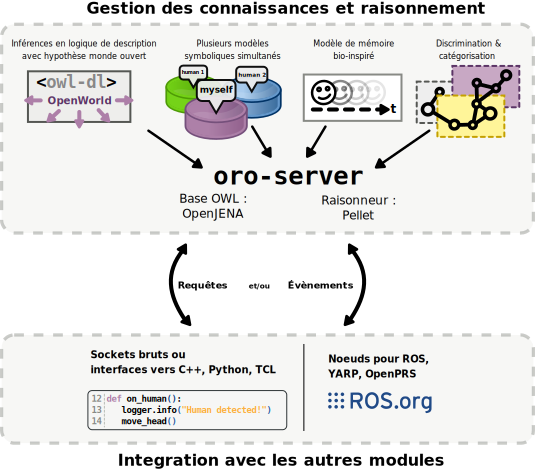
\includegraphics[width=0.75\columnwidth]{oroserver/oro_architecture_functional-fr.pdf}
  \caption{Aperçu fonctionnel de l'architecture d'ORO.}
  \label{fig|oro-overview}
\end{figure}

L'une des particularités importante de ce système est qu'il permet de gérer
plusieurs modèles symboliques en parallèle. Chacun de ces modèles est
indépendant et cohérent d'un point de vue logique, ce qui permet de raisonner
en ce plaçant dans des \emph{perspectives cognitives} différentes sur le monde.
Ces perspectives peuvent être globalement incohérentes : par exemple, un objet
peut être visible par le robot, mais invisible pour l'homme. Cet objet aura
simultanément les propriétés \concept{isVisible \textit{true}} et
\concept{isVisible \textit{false}} dans deux modèles différents.

{\sc Spark} (figure~\ref{fig|spark}) est un environnement 3D temps réel
(développé hors du cadre de cette thèse) qui permet de calculer en ligne
plusieurs propriétés géométriques dépendantes de la perspective de chaque agent
(on parle de \emph{prise de perspective}) et qui nourrit les modèles abrités
par ORO avec ces propriétés symboliques (les faits effectivement calculés sont
présentés au chapitre~\ref{sect|situ}).

\begin{figure}
\centering
  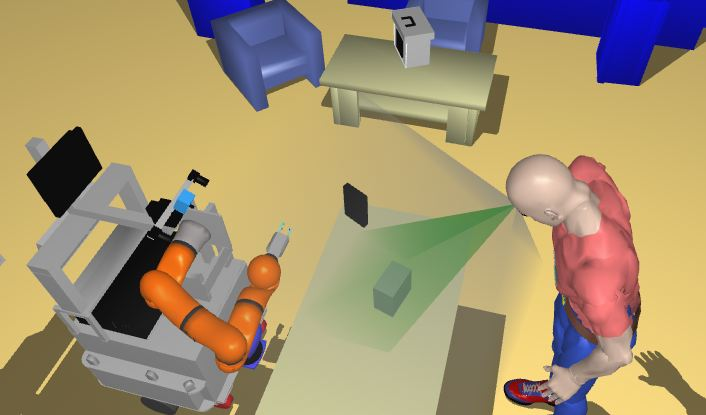
\includegraphics[width=0.6\columnwidth]{spark/looks.jpg}

  \caption{L'environnement 3D dans {\sc Spark}. Dans cet exemple, le logiciel
  calcule quels objets sont visible pour l'homme à partir de cônes de
  visibilité et d'attention.}

  \label{fig|spark}
\end{figure}

Le fait de maintenir un modèle symbolique indépendant par agent nous permet de
considérer le robot doté d'une \emph{théorie de l'esprit}~\cite{Leslie2000}
simple : le robot devient capable de représenter les modèles mentaux,
éventuellement divergents, des autres agents intelligents avec lesquels il
interagit.

Ces modèles multiples peuvent aussi être vus comme autant de \emph{cadres
d'interprétation} de la connaissance, et donc comme autant d'éléments de
contexte.

ORO propose d'autres outils cognitifs aux modules du robot : outre son rôle de
base de fait (qui inclut, come nous l'avons brièvement mentionné, l'ajout, la
retractaction, la mise à jour de faits symboliques, l'interrogation de la base
par plusieurs mécanismes de requêtes, des outils de parcours taxonomique --
classes parentes, instances, propriétés d'un concept, ...), le serveur fournit
des mécanismes de classification des concepts (à partir d'un ensemble de
concepts, déterminer la meilleure partition), de discrimination (quelles
propriétés d'un ensemble de concept permettent de les distinguer de la manière
la plus efficace) ou encore de mémoire (certains faits peuvent être associés à
un profil de mémoire déterminant la durée pendant laquelle ils sont gardés).

\subsection*{Integration dans les architectures robotiques}

ORO a été intégré dans plusieurs architectures robotiques (les expériences
présentées au chapitre~\ref{sect|experimental-evaluation} en témoignent
précisément).

D'un point de vue architectural, la principale contribution de notre système
est le mécanisme évènementiel \emph{au niveau sémantique} qu'il introduit. Un
exemple d'évènement sémantique a déjà été fournit précédemment : les composants
de supervision du robot peuvent demander à être notifiés lorsque certaines
conditions logiques sont vérifiées par ORO (comme la présence d'un fait
correspondant à l'exemple {\tt [* type Human, * looksAt myself, * isSitting
true]} que nous proposions ci-dessus). Le sous-système s'inscrivant à un tel
évènement accède de manière indirecte et abstraite aux modules de perception
(qui détectent la présence d'un homme et sa posture) tout en bénéficiant le cas
échéant et de manière transparente des capacités de raisonnement symbolique de
la base de fait.

\begin{figure*}[thpb]
  \centering
  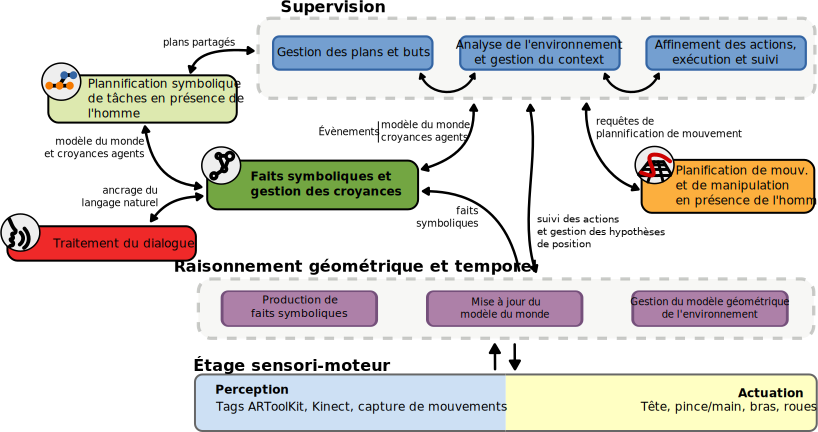
\includegraphics[width=\columnwidth]{integration/architecture_overview-fr.pdf}

  \caption {Schéma de l'architecture logicielle déployée sur les robots PR2 et
  Jido, deux robots de services interagissant avec des hommes au LAAS-CNRS. Le
  serveur ORO apparait en vert, au milieu.}

  \label{fig|archi}
\end{figure*}

Comme l'illustre la figure~\ref{fig|archi}, l'intégration de ORO ne se limite
pas aux modules de supervision. Nous avons déjà mentionné le module de
raisonnement géométrique {\sc Spark} qui calcule et fournit un ensemble de fait
symbolique issus de l'analyse de l'environement du robot. ORO fournit aussi le
modèle symbolique du monde et des croyances des agents au planificateur
symbolique de tâche {\sc Hatp}, et joue un rôle clé dans le traitement de la
langue naturelle.

Le traitement du dialogue, longuement détaillé dans le corps de la thèse au
chapitre~\ref{chapt|dialogs}, repose sur une interaction forte avec la base de
connaissances : ORO sert non seulement à stocker le résultat de l'analyse de
l'interaction verbale (comme l'expression un désir, ou une nouvelle assertion
sur le monde), mais surtout à fournir le modèle de connaissance nécessaire à
\emph{l'ancrage} sémantique des phrases. Ainsi, une phrase comme \og
Apporte-moi le livre \fg prête à confusion dès que deux livres sont présents
dans la scène. Le module de traitement du dialogue traite l'ambiguité en
vérifiant dans ORO quels objets sont effectivement connus de l'homme, quels
sont ceux qui sont visibles, et le cas échéant, formule une question en se
basant sur les proprités discriminantes de l'ensemble des livres présents.


\subsection*{Instantiation de la connaissance : l'ontologie OpenRobots Common-Sense}
\label{sect|oro-commonsense}

La plateforme ORO est composée du serveur que nous venons de présenté et d'une
ontologie dite de \emph{sens commun} (\emph{common-sense}) qui sert de base de
connaissances \textit{a priori} au robot.

\begin{figure}
    \centering
    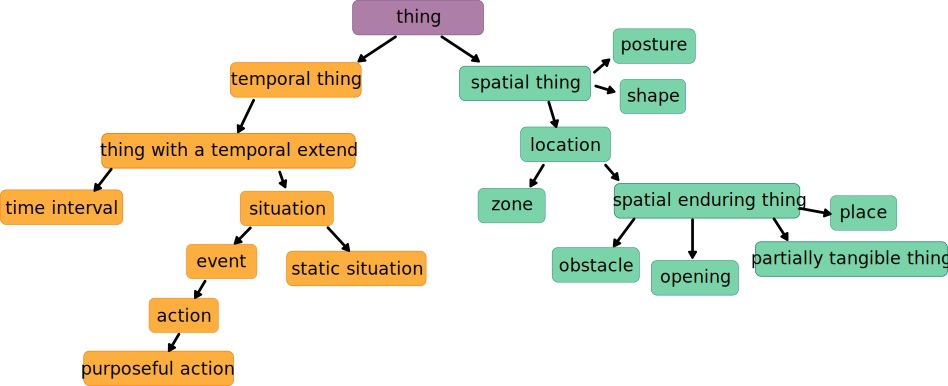
\includegraphics[scale=0.6]{oro/top_tbox.pdf}

    \caption{Extrait de la partie supérieure de l'ontologie common-sense de
    ORO. Tous ces concepts appartiennent à l'espace de nommage de l'ontologie
    mère {\sc OpenCyc}.}

    \label{fig|upper_tbox}
\end{figure}

Cette ontologie a été conçue sur la base de deux principes : couvrir nos
besoins expérimentaux, et se conformer autant que possible à l'ontologie
standard {\sc OpenCyc} afin de garantir une inter-opérabilité du modèle de
connaissance du robot sur le long terme.

Ceci nous a conduit à un processus de développement bidirectionel :
\textit{bottom-up} en ce qui concerne le choix des concepts à modéliser,
\textit{top-down} en ce qui concerne la partie supérieure de la taxonomie comme
illustré dans la figure~\ref{fig|upper_tbox}.

Cette même figure fait par ailleurs apparaitre une disjonction fondamentale
dans le modèle des connaissances induit par ORO entre entités
\emph{temporelles} et \emph{spatiales}.

Le chapitre~\ref{sect|oro-commonsense} de la thèse entre dans certains détails
du modèle de connaissance que nous n'abordons pas dans ce résumé.

\section{Évaluation expérimentale}


This chapter was focused on the evaluation, from two different perspectives.

First, we have presented a large table that summarises how the main features
and requirements of knowledge representation systems identified at
chapter~\ref{chapt|krs} are matched by the existing implementations. We have
discussed the successes and limits of the current state of the art based on a
list of high-level requirements established from McCarthy and Roy proposals
towards more advanced artificial cognition.

Amongst the fields that are identified as requiring more research efforts,
non-monotonic representations, explaining of the mental state and the mental
processes, and context representation represent largely open challenges.

Then, we have presented several experimental frameworks and experiments.

MORSE, a simulator with strong HRI capabilities has been briefly presented.
Three case-studies demonstrating the classification and learning capabilities
of ORO have been then introduced. Three larger experiments, involving verbal
interaction, task planning and execution control have been then presented and
explained.

Finally, we have mentioned the Roboscopie theatre performance as an unusual
experimental setup, targeted at a general public audience. We see it as a way
to materialize and discuss the relationships between the robots and the humans,
and to address these questions ``in the open'', outside of the closed frame of
the laboratory.





